\begin{document}
Pel que fa a l'anàlisi de costos, s'ha intentat segregar segons els diferents paràmetres on el sistema es pot derivar, que són:
\begin{itemize}
	\item La mida del sistema agregat, és a dir, el nombre de comptadors d'un barri.
	\item L'algorisme emprat per tal de calcular el logaritme discret.
\end{itemize}
No obstant això, anteriorment s'ha especificat certes propietats que comporta el sistema:
\label{sec:dataset}
\begin{itemize}
	\item Les simulacions s'han dut a terme usant un processador \texttt{AMD Ryzen 7 4800H @ 2.900GHz} de $16$ nuclis. S'ha realitzat 150 iteracions en cada simulació i s'ha fet la mitjana sobre aquestes dades per trobar un valor representatiu.
	\item Es considera que entre ronda i ronda hi haurà, com a mínim, un interval de 15 minuts, és a dir, la lectura que es passarà correspondrà al consum dels últims 15 minuts.
	\item Per tal de no sobrecarregar l'algoritme del logaritme discret, les lectures dels comptadors han de tenir un cert grau de control en la seva mida en bits.\\
	 Primer, es va pensar realitzar l'anàlisi amb lectures pseudoaleatòries. Per aquesta raó, està creada la classe \texttt{RandomConsumption}, que enviava un enter positiu aleatori de, com a màxim, 13 bits. Aquesta classe ens servirà per poder comparar els diferents protocols o realitzar funcions estadístiques, ja que les lectures no es comportaran diferent segons la ronda quan s'envien.\\
	 No obstant això, amb la intenció de tenir una simulació més realista, s'ha buscat un \textit{dataset} que ens permeti visualitzar el consum elèctric d'una llar \cite{kaggle-consumption} i crear lectures més properes a les reals. Aquestes dades ens serviran per poder veure fins quan el cost de realitzar el logaritme discret és factible.\\
	 Les dades trobades aporten el consum elèctric amb una freqüència de mostreig d'un minut durant aproximadament 4 anys en tres espais diferents de la llar, tal com es pot apreciar a la \textit{Taula \ref{tab:ex-kaggle}}.
	\begin{table}[H]
		\centering
			\begin{tabular}{llrrr}
				\toprule
				{} &           date\_time &  Sub\_metering\_1 &  Sub\_metering\_2 &  Sub\_metering\_3 \\
				\midrule
				0 & 2006-12-16 17:24:00 &             0.0 &             1.0 &            17.0 \\
				1 & 2006-12-16 17:25:00 &             0.0 &             1.0 &            16.0 \\
				2 & 2006-12-16 17:26:00 &             0.0 &             2.0 &            17.0 \\
				3 & 2006-12-16 17:27:00 &             0.0 &             1.0 &            17.0 \\
				4 & 2006-12-16 17:28:00 &             0.0 &             1.0 &            17.0 \\
				...\\
				\bottomrule
			\end{tabular}
		\caption{Primeres files del dataset.}
		\label{tab:ex-kaggle}
	\end{table}
	Primer, s'han tractat les dades agregant els consums dels diferents espais per trobar el consum total de la llar. Seguidament, un cop tenint el consum de la llar agregat, es realitza la mitjana d'aquest valor en funció del temps, és a dir, la mitjana de tots els dies en funció de l'hora i el minut en què s'ha realitzat la lectura. Una part del resultat obtingut es mostra a la \textit{Taula \ref{tab:ex-kaggle-mean}}, com a exemple.
	\begin{table}[H]
		\centering
		\begin{tabular}{lrrr}
			\toprule
			{} & hour & min & consumption mean \\
			\midrule
			0 &    0 &   0 &    4.537868 \\
			1 &    0 &   1 &    4.524544 \\
			2 &    0 &   2 &    4.568022 \\
			3 &    0 &   3 &    4.599579 \\
			4 &    0 &   4 &    4.600281 \\
			5 &    0 &   5 &    4.666199 \\
			6 &    0 &   6 &    4.443198 \\
			7 &    0 &   7 &    4.525947 \\
			8 &    0 &   8 &    4.596073 \\
			...\\
			\bottomrule
		\end{tabular}
	\caption{Primeres files del dataset transformat realitzant la mitjana}
	\label{tab:ex-kaggle-mean}
	\end{table}
	   Així doncs, es pot visualitzar la mitjana trobada pel consum elèctric total de la llar en funció de l'horari de la següent forma:
\begin{figure}[H]
	\centering
	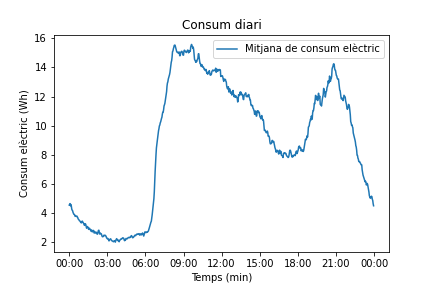
\includegraphics[width=8cm]{imgs/cost/consumptionmin.png}
	\caption{Mitjana de consum diari.}
	\label{fig:consumptionmin1}
\end{figure}
Per tal de variar les lectures entre diferents comptadors, s'ha creat una cota màxima i una cota mínima per establir un rang de possibilitats.
\begin{figure}[H]
	\centering
	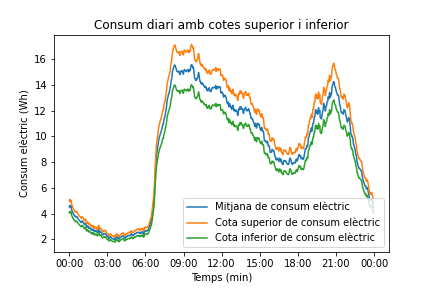
\includegraphics[width=8cm]{imgs/cost/consumptionmin2.png}
	\caption{Mitjana de consum diari amb cotes superior i inferior.}
	\label{fig:consumptionmin2}
\end{figure}
Finalment,  s'han agregat els consums de 15 minuts en 15 minuts, ja que la lectura es passarà en intervals de 15 minuts, com ja s'ha mencionat anteriorment. D'aquesta manera, cada quart d'hora correspon a una classe d'equivalència. \\
En conclusió, es pot afirmar que agafant un nombre pseudoaleatori dins del rang possible corresponent a cada ronda, es pot acabar generant un dia de lectures més o menys fidel a la realitat. No obstant això, cal esmentar que s'ha modificat lleugerament la cota superior per tal de crear més variació entre comptadors, tal com es pot veure a la \textit{Figura \ref{fig:consumption2}}.
\begin{figure}[H]
	\centering
	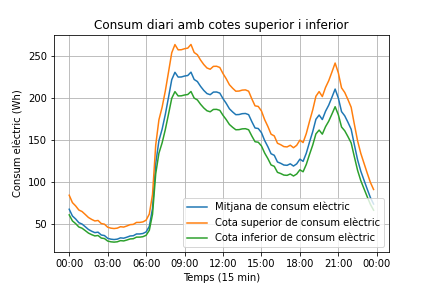
\includegraphics[width=8cm]{imgs/cost/consumption2.png}
	\caption{Gràfica de lectures amb cotes superior i inferior.}
	\label{fig:consumption2}
\end{figure}
Com es pot observar, les lectures mai seran d'una mida superior a $13$ bits, ja que $log_2(v_{max}) = log_2(263) = 8.04$. Sabent això, el missatge xifrat agregat serà d'una llargada màxima de $|D_2|_{max} = 8 + \lceil log_2(N) \rceil$ sent $N$ el nombre de comptadors intel·ligents al barri.
\end{itemize}
Es pot veure el tractament del \textit{dataset} i de les dades obtingudes en l'anàlisi de cost en el repositori remot \cite{lab-recsi} implementat en \texttt{python3} usant \texttt{jupyter notebooks}. Per tal d'analitzar i veure gràficament les dades que ens aportaven els costs, s'han usat les següents tecnologies pel tractament de dades: \texttt{pandas}, \texttt{numpy} i \texttt{matplotlib}.
\section{Algorismes de computació del logaritme discret}
El primer que es voldrà analitzar seran els diferents algoritmes implementats que realitzen el logaritme discret, que són un total de tres:
\begin{itemize}
	\item Pollard's Lambda, descrit a la \textit{Secció \ref{sec:pollards}}.
	\item Algoritme de força bruta \texttt{BruteForce}, on el generador passa pels possibles elements del grup fins a trobar la potència. Aquest algoritme es va utilitzar per realitzar diversos tests i s'ha cregut encertat comparar-lo amb el Pollard's Lambda.
	\item Algoritme \textit{singleton} de força bruta \texttt{HashedAlgorithm}, on es realitza un cop l'algoritme per guardar les relacions entre tots els elements i la seva respectiva potència. De manera que, si es carrega la classe abans, l'únic cost a l'hora de realitzar el logaritme discret serà l'accés a memòria. No obstant el cost del temps és més reduït, la memòria que ocupa és bastant gran i es necessita un temps inicial per construir la taula. Al final, el que tindrem a l'hora de cridar el mètode serà un \textit{HashMap} que, donat un element $a \in \mathbb{Z}_p$ o  $A \in E(\mathbb{Z}_p)$ ens retornarà la seva clau $k$, sabent que:
	\[g^k = a ,\quad \textrm{ usant  }\ \mathbb{Z}_p\]
	\[G \cdot k = A,\quad \textrm{ usant  }\ E(\mathbb{Z}_p)\]
\end{itemize}
El generador de lectures usat és el \texttt{RandomConsumption} per tenir la mateixa configuració pel que fa a la llargada dels missatges, ja sigui en \textit{Key Establishment} com \textit{Consumption Transmission}. 
A l'hora d'analitzar en funció de l'algoritme \texttt{BruteForce}, a causa del temps que requereix per realitzar el logaritme discret, només s'ha repetit el cas 100 cops per cada configuració. Un dels motius perquè la fase \textit{Consumption Transmission} és un pèl més costosa que \textit{Key Establishment} és perquè a l'hora de passar l'últim fragment de les claus, aquest té un valor més petit. Això causa que es resolgui el logaritme discret més ràpidament.
	\begin{table}[H]
		\centering
		\begin{tabular}{lrrrrrrr}
			\centering
			&\multicolumn{7}{l}{\centering Temps (ms)}\\
			\toprule
			Num meters: &           3  &       4  &           5  &            8  &            16 & 32 & 64\\
			\midrule
			ct &  13033.5 &  17353.66 &  21732.06 &  37016.33 &  78411.33 &   163313.4 &  350156.66 \\
			ke &  12034.19 &  17373.6 &  21035.46 &  34766.13 &  73173.26 &  153523.73 &  329552.0 \\
			\bottomrule
		\end{tabular}
		\caption{Cost experimental del protocol usant \texttt{BruteForce}.}
		\label{tab:brute}
	\end{table}
Els resultats en \texttt{PollardsLambda} i \texttt{HashedAlgorithm}, que es mostren a la \textit{Taula \ref{tab:pollards}} i la \textit{Taula \ref{tab:hashed}} respectivament, són molt més prometedors i verifiquen que el logaritme discret, en cas de no estar implementat de manera eficient, pot generar un coll d'ampolla.

\begin{table}[H]
	\centering
	\begin{tabular}{lrrrrrrrrr}
		\centering
		&\multicolumn{9}{l}{\centering Temps (ms)}\\
		\toprule
		Num meters: &           3  &       4  &           5  &            8  &              16  &         32  &         64  &      128 &     192 \\
		\midrule
		ct &  926.4 &  926.27 &  949.4 &  976.67 &  964.8 &  1134.0 &  1221.33 &  1480.6 &  1667.53 \\
		ke &  970.67 &  971.73&  919.13&  1032.53 &  1136.6 &  1484.06 &  2071.8 &  2794.73 &  3589.13 \\
		\bottomrule
	\end{tabular}
	\caption{Cost experimental del protocol usant \texttt{PollardsLambda}.}
	\label{tab:pollards}
\end{table}
\begin{table}[H]
	\centering
	\begin{tabular}{lrrrrrrrrr}
		\centering
		&\multicolumn{9}{l}{\centering Temps (ms)}\\
		\toprule
		Num meters: &           3  &       4  &           5  &            8  &              16  &         32  &         64  &      128 &     192 \\
		\midrule
		ct &  206.53 &  224.8 &  231.6 &  225.67 &  227.0 &  320.27 &  506.07 &  754.0 &  993.27 \\
		ke &  382.0 &  405.66 &  422.4 &  452.4 &  578.4 &  1082.866 &  1649.33 &  2459.53 &  3183.33 \\
		\bottomrule
	\end{tabular}
	\caption{Cost experimental del protocol usant \texttt{HashedAlgorithm}.}
	\label{tab:hashed}
\end{table}
No obstant això, es pot observar que la funció de cost en tots els algoritmes és lineal i no exponencial, tal com hauria de ser. Això és degut a les especificacions del processador, ja que només té 4 nuclis i no permet que els comptadors treballin de manera simultània. Això provoca que, a l'usar un nombre de processos més elevat que el de nuclis o \textit{threads virtuals}, en cas que en tingués, no es pot realitzar una simulació paral·lela. Gràcies a això també es pot explicar per què la fase \textit{KE}, que és la que comporta més comunicació entre comptadors i subestació, és la fase més costosa usant els algoritmes \texttt{HashedAlgorithm} i \texttt{PollardsLambda}, on el cost del logaritme és més baix.
\\
\\
 A la \textit{Figura \ref{fig:comparisons}} es compara el cost del protocol en funció de \texttt{PollardsLambda} i \texttt{HashedAlgorithm}. No s'ha pogut comparar en aquest gràfic \texttt{BruteForce}, doncs el cost és molt més alt.
 Mentre que a la \textit{Figura \ref{fig:algorithms}} es pot veure el resultat de les taules de manera més gràfica.
\begin{figure}[H]
	\centering
	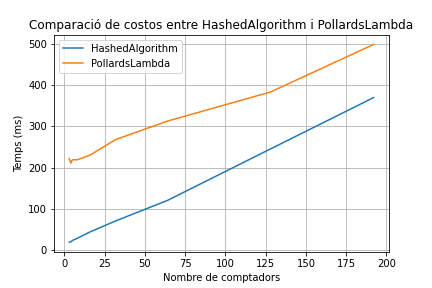
\includegraphics[width=9cm]{imgs/cost/comp-hashed-pollards.png}
	\caption{Comparació de rendiment del protocol entre els algoritmes \texttt{HashedAlgorithm} i \texttt{PollardsLambda}.}
	\label{fig:comparisons}
\end{figure}
\begin{figure}[H]
	\centering
	\begin{subfigure}[b]{0.47\textwidth}
		\centering
		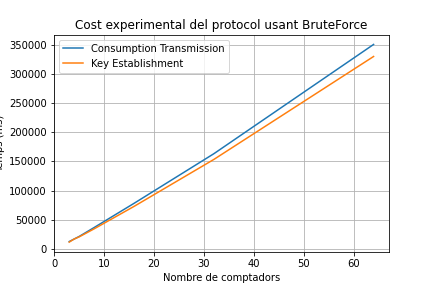
\includegraphics[width=\textwidth]{imgs/cost/brute.png}
	\end{subfigure}
\begin{subfigure}[b]{0.47\textwidth}
	\centering
	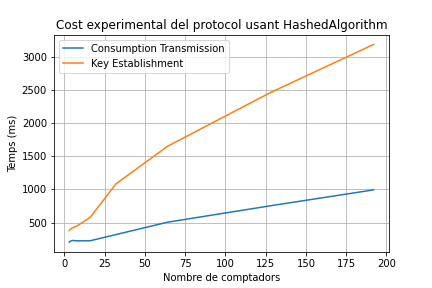
\includegraphics[width=\textwidth]{imgs/cost/hashed.png}
\end{subfigure}
\begin{subfigure}[b]{0.47\textwidth}
	\centering
	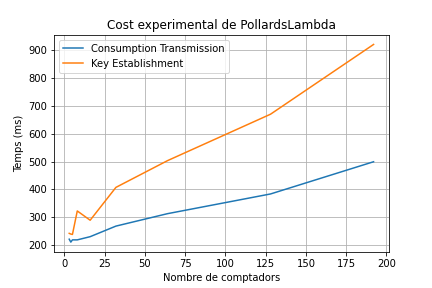
\includegraphics[width=\textwidth]{imgs/cost/pollards.png}
\end{subfigure}
	\caption{Costos experimentals de les fases en funció dels algoritmes}
	\label{fig:algorithms}
\end{figure}
Per tal de verificar que el cost del logaritme discret és exponencial i veure més detalladament el cost de cada algoritme, s'ha analitzat el cost de l'algoritme en funció del nombre de bits del missatge, d'aquesta manera, perdem el coll d'ampolla a la sincronia. A la \textit{Figura \ref{fig:cost-algo}}, es pot observar com \texttt{PollardsLambda} té un rendiment molt més bo, aconseguint realitzar el logaritme discret d'un missatge de 24 bits en el mateix temps que ho fa \texttt{BruteForce} amb un de 13 bits.
\begin{figure}[H]
	\centering
	\begin{subfigure}[b]{0.48\textwidth}
		\centering
		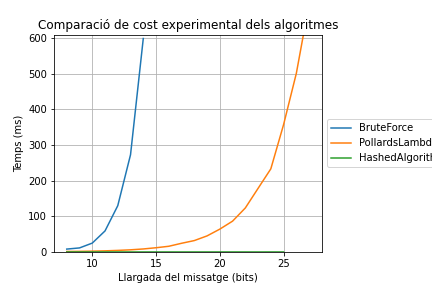
\includegraphics[width=7cm]{imgs/cost/algoritmes-cost.png}
	\end{subfigure}
	\begin{subfigure}[b]{0.48\textwidth}
	\centering
	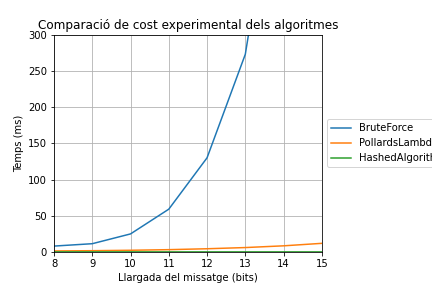
\includegraphics[width=7cm]{imgs/cost/algoritmes-cost2.png}
	\end{subfigure}
	\caption{Comparació dels costos experimentals dels algoritmes en funció del nombre de bits.}
	\label{fig:cost-algo}
\end{figure}
Encara que l'algoritme cachejat tingui un cost teòric $\mathcal{O}(1)$ a l'hora de buscar el logaritme discret, té una càrrega inicial exponencial segons el nombre de bits que es vulgui agafar. Si es busca algun logaritme el resultat el qual s'escapi d'aquests bits, aquest no el podrà trobar.
\begin{figure}[H]
	\centering
	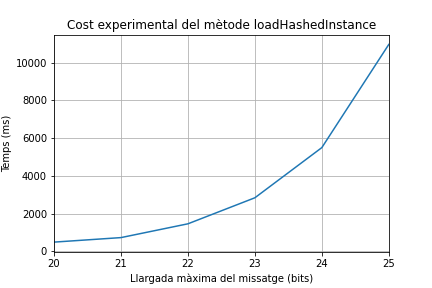
\includegraphics[width=9cm]{imgs/cost/pollardslambda.png}
	\caption{Cost experimental del mètode \texttt{loadHashedInstance}.}
	\label{fig:pollardslambda}
\end{figure}
A més a més, és important l'ús de la memòria principal en aquest tipus d'algoritmes, ja que guardant $2^{20}$ relacions, s'ha necessitat \texttt{1 GB} en memòria.
\section{Comparació de \cite{recsi} i \cite{busom}}
S'ha comparat el cost en temps dels protocols \cite{recsi} i \cite{busom} en funció del nombre de comptadors i de missatges. Encara que \cite{busom} té un establiment de claus més senzill que \cite{recsi}, aquest últim té una comunicació menys costosa a la fase \textit{Consumption Transmission}, per aquest motiu, es pot deduir que, en el cas de tenir moltes rondes, és aconsellable usar \cite{recsi}. No obstant això, veiem a la \textit{Figura \ref{fig:prottime16}}, que en la simulació en comunitats de $16$ comptadors, no es pot apreciar una millora en \cite{recsi}. Això és a causa que la simulació s'ha realitzat en un mateix ordinador i el cost en temps del pas de lectures dels comptadors a la subestació és negligible, cosa que no es pot assumir que, en un cas real, existeixi sempre aquesta propietat.
\begin{figure}[H]
	\centering
	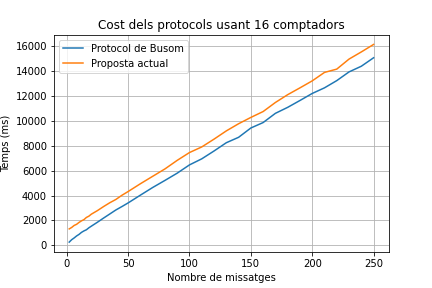
\includegraphics[width=9cm]{imgs/cost/16compt.png}
	\caption{Costos experimentals dels protocols \cite{recsi} i \cite{busom} en comunitats de 16 comptadors.}
	\label{fig:prottime16}
\end{figure}
Per aquest motiu, s'ha realitzat analitzat en comunitats de 32 comptadors. Així doncs, l'ordinador no pot realitzar la simulació de manera paral·lela. D'aquesta forma privem a la subestació d'una comunicació eficient, ja que tarda més a rebre totes les lectures en una ronda. Es pot observar a la \textit{Figura \ref{fig:prottime32}} que, a mesura que el nombre de missatges augmenta, \cite{recsi} es torna més eficient.
\begin{figure}[H]
	\centering
	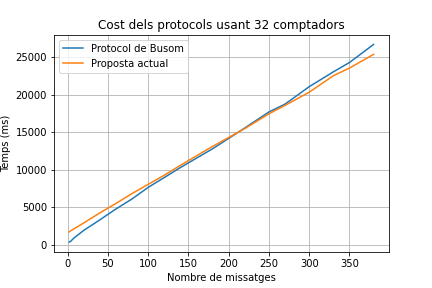
\includegraphics[width=9cm]{imgs/cost/32compt.png}
	\caption{Costs experimentals dels protocols \cite{recsi} i \cite{busom} en comunitats de 32 comptadors.}
	\label{fig:prottime32}
\end{figure}

En conclusió, es pot observar que, en el cas de tenir poques rondes en la fase \textit{Consumption Transmission}, \cite{busom} és una millor proposta al tenir una configuració de claus més senzilla. 
Per altra banda, si es sap que la comunicació entre comptadors i subestació és costosa o triga massa  i es pot tenir un nombre de rondes en \textit{Consumption Transmission} considerable, és més aconsellable usar \cite{recsi}, perquè el cost es veurà menys afectat usant aquest sistema. Sigui $R$ el nombre de rondes en la fase \textit{Consumption Transmission}, podem dir que si la següent avaluació és certa, és millor usar \cite{busom}.
\[Cost_2(R) < Cost_1(R)\]
Per desenvolupar més aquesta inequació, podem partir el cost de cada protocol en la suma de costos de les seves fases.
\[Cost_{KE_2} + Cost_{CT_2}(R) <  Cost_{KE_1} + Cost_{CT_1}(R)\]
La fase \textit{Key Establishment} de \cite{recsi}, a més a més, depèn del nombre de fragments de la clau privada que han d'enviar els comptadors. Aquests fragments estan determinats per l'ordre de la corba i la mida en bits del que es vol transmetre, que està estipulat que sigui $13$ per tal de no elevar gaire el cost de realitzar el logaritme discret en cada iteració. D'aquesta manera, es pot veure que el nombre de fragments és: 
\[|Fragments| = \frac{\textrm{ordre de la corba}}{\#\textrm{fragment}_2} = \frac{\textrm{ordre de la corba}}{13}\]
Com que la fase \textit{KE} de \cite{recsi} s'usa el protocol \cite{busom}, es pot dir de manera general que:
\[Cost_{KE_1} = Cost_2(|Fragments|)\]
Així doncs, substituint veiem que:
\[Cost_{KE_2} + Cost_{CT_2}(R) <  Cost_{2}(|Fragments|) + Cost_{CT_1}(R)\]
A més a més, sabem que, el cost de la fase de \textit{Consumption Transmission} de \cite{busom} és més elevat que el de \cite{recsi} per culpa del cost de comunicació. Llavors, podem assumir, simplificant una mica el problema sense tenir en compte altres possibles tipus de factors, que hi ha una proporció entre les dues fases en funció d'aquest cost.
\[Cost_{CT_2}(R) = Cost_{CT_1}(R) \cdot k_{\textrm{comunicació}}, \qquad k_{\textrm{comunicació}} \ge 1\]
Substituint el cost de la fase de \textit{Consumption Transmission} de \cite{busom} en l'inequació veiem que:
\[Cost_{KE_2} + Cost_{CT_1}(R) \cdot k_{\textrm{comunicació}} \le  Cost_{2}(|Fragments|) + Cost_{CT_1}(R)\]
Podem observar que, si $k_{\textrm{comunicació}} = 1$, és  a dir, el cost de comunicació és negligible, és millor usar \cite{busom}, ja que el cost de la fase \textit{Key Establishment} és més petit que el cost del mateix protocol $Cost_{KE_2} \le Cost_{2}$. Per altra banda, si $k_{\textrm{comunicació}} > 1$, la tria depèn, bàsicament, del nombre de rondes $R$, ja que, tard o d'hora, com que la fase de \textit{Consumption Transmission} de \cite{recsi} és menys costosa que \cite{busom}, aquest primer tindrà un avantatge a partir d'un nombre determinat de rondes.
\[Cost_{KE_2} <  Cost_{2}(|Fragments|) + Cost_{CT_1}(R) \cdot (1 - k_{\textrm{comunicació}})\]
Es pot entendre $Cost_{CT_1}(R) \cdot (1 - k_{\textrm{comunicació}})$ com la diferència en el temps entre les fases de \textit{Consumption Transmission} dels dos protocols en un determinat nombre de rondes $R$. La inequació es pot desenvolupar una mica més, partint el cost del protocol \cite{busom}, sabent que
$Cost_{2}(|Fragments|) = Cost_{KE_2} + Cost_{CT_2}(|Fragments|)$.
\[Cost_{KE_2} <  Cost_{KE_2} + Cost_{CT_2}(|Fragments|) + Cost_{CT_1}(R) \cdot (1 - k_{\textrm{comunicació}})\]
Finalment, podem simplificar treient $Cost_{KE_2}$ de la inequació, obtenint:
\[0 < Cost_{CT_2}(|Fragments|) + Cost_{CT_1}(R) \cdot (1 - k_{\textrm{comunicació}})\]
D'aquesta manera, podem concloure que si $Cost_{CT_2}(|Fragments|) + Cost_{CT_1}(R) \cdot (1 - k_{\textrm{comunicació}})$ és positiu, serà millor usar \cite{ busom}. Si el resultat dóna negatiu, la millor opció serà \cite{recsi}, ja que el cost de comunicació és suficientment elevat per ser més ràpid que \cite{busom}.  De forma resumida, si $\ \ |Cost_{CT_1}(R) \cdot (1 - k_{\textrm{comunicació}})| > Cost_{CT_2}(|Fragments|)$ la millor opció serà \cite{recsi}.
\section{Simulació usant el dataset}
Per comprovar d'una altra manera que hi ha una correlació entre la mida dels missatges i el temps en el protocol, s'ha usat el \textit{dataset} mencionat a l'inici de la \textit{Part \ref{sec:dataset}}. Per tal de realitzar-ho, s'ha comparat el cost que té la subestació en rebre la lectura general en les diferents rondes de la fase \textit{Consumption Transmission}. D'aquesta manera, es troba una funció semblant a la que es troba en les lectures dels consumidors, tal com es veu a la \textit{Figura \ref{fig:cost-kaggle}}. Cal dir, que per veure els resultats de manera més significativa, s'ha usat $200$ simulacions de comunitats de $32$ comptadors\footnote{D'aquesta manera, la llargada màxima del missatge augmenta 4 bits.} i fent ús de l'algoritme \texttt{BruteForce} per realitzar el logaritme discret. Per aquesta raó, no s'ha usat el \texttt{HashedAlgorithm}, ja que aquest no augmenta en cada ronda sinó al principi, abans de la fase \textit{Key Establishment}.
\\
\\
En el gràfic del cost del protocol en funció de la ronda, es pot observar un pic a la primera ronda. Això és deu possiblement a què és la primera iteració de la fase \textit{Consumption Transmission} i s'ha de carregar el codi a memòria, cosa que comporta un cost en el temps, tant pels comptadors com per la subestació. Per aquest motiu, aquest pic només passa en la primera iteració. Aquest comportament també passa usant els altres algoritmes per realitzar el logaritme discret.
\begin{figure}[H]
	
	\centering
	\begin{subfigure}[b]{0.48\textwidth}
		\centering
		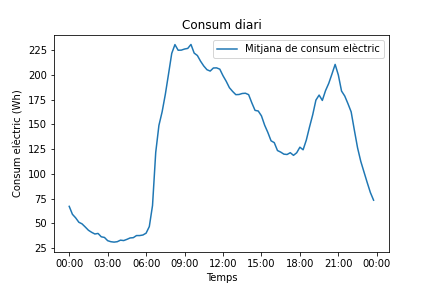
\includegraphics[width=7cm]{imgs/cost/consumption.png}
	\end{subfigure}
	\begin{subfigure}[b]{0.48\textwidth}
		\centering
		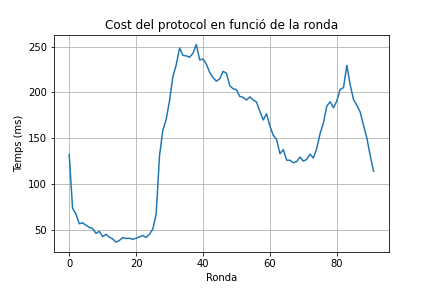
\includegraphics[width=7cm]{imgs/cost/16compt-dataset.png}
	\end{subfigure}
	\caption{Comparació entre la gràfica de consum i gràfica del cost en temps del protocol segons la ronda.}
	\label{fig:cost-kaggle}
	\centering
\end{figure}
\end{document}